\documentclass[border=10pt]{standalone}
\usepackage[T1]{fontenc}
\usepackage{tikz}
\usetikzlibrary{arrows.meta, positioning, fit, backgrounds, calc, shapes.geometric}

\definecolor{node0bg}{HTML}{E8F5E9}
\definecolor{node1bg}{HTML}{E3F2FD}
\definecolor{node2bg}{HTML}{FFF3E0}
\definecolor{node3bg}{HTML}{F3E5F5}
\definecolor{collector}{HTML}{1565C0}
\definecolor{storage}{HTML}{6A1B9A}
\definecolor{observ}{HTML}{E65100}
\definecolor{svccolor}{HTML}{2E7D32}
\definecolor{n3svccolor}{HTML}{7B1FA2}
\definecolor{arrow-otlp}{HTML}{1565C0}
\definecolor{arrow-query}{HTML}{E65100}
\definecolor{arrow-file}{HTML}{6A1B9A}
\definecolor{arrow-kafka}{HTML}{D84315}
\definecolor{arrow-cross}{HTML}{6A1B9A}

\begin{document}
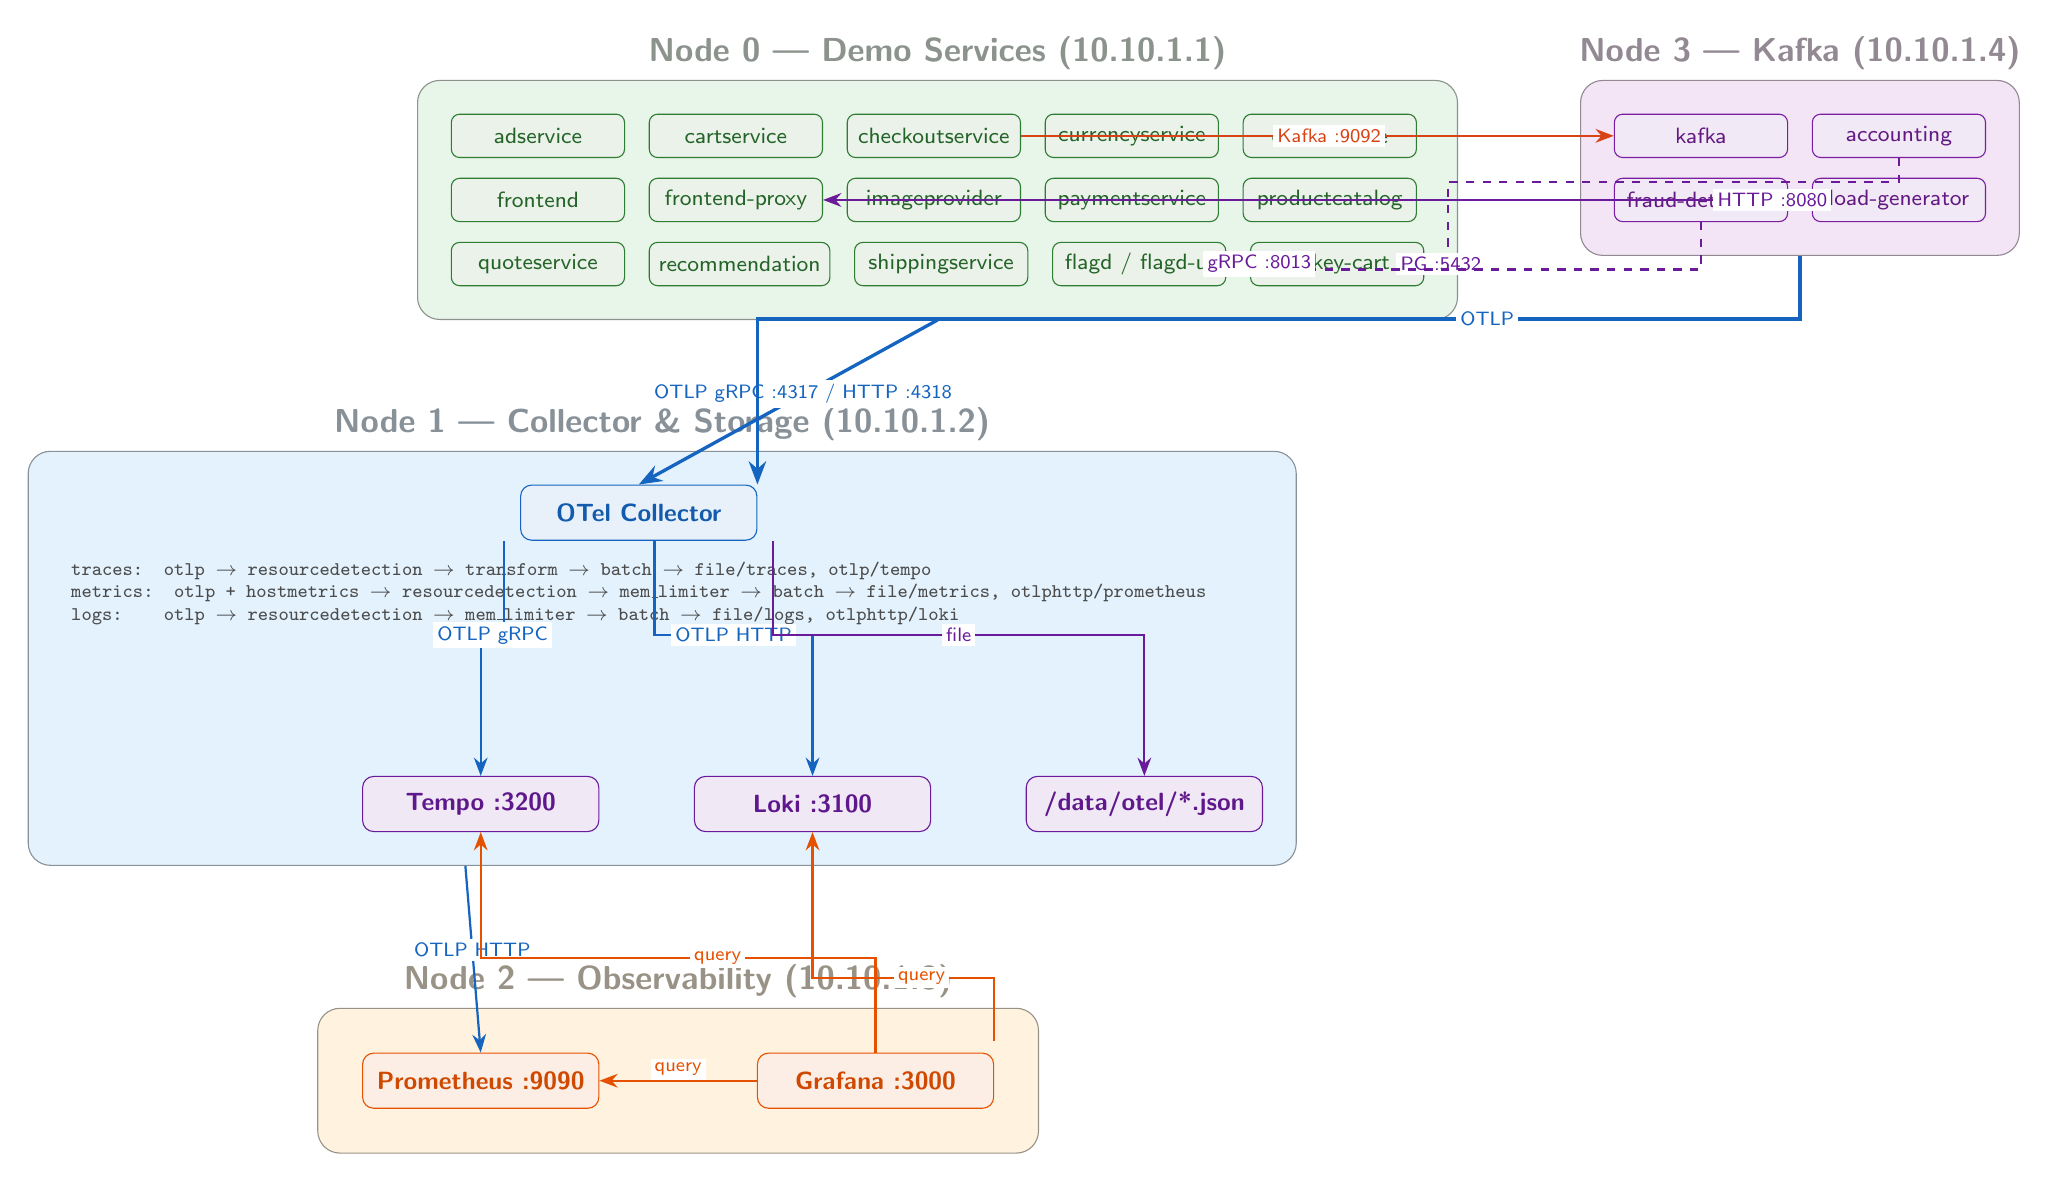
\begin{tikzpicture}[
    >=Stealth,
    node distance=1.2cm and 2.5cm,
    svc/.style={draw=svccolor, fill=svccolor!10, rounded corners=3pt,
                font=\footnotesize\sffamily, minimum width=2.2cm, minimum height=0.55cm,
                text=svccolor!80!black},
    n3svc/.style={draw=n3svccolor, fill=n3svccolor!10, rounded corners=3pt,
                font=\footnotesize\sffamily, minimum width=2.2cm, minimum height=0.55cm,
                text=n3svccolor!80!black},
    component/.style={draw=#1, fill=#1!10, rounded corners=4pt,
                      font=\small\sffamily\bfseries, minimum width=3cm, minimum height=0.7cm,
                      text=#1!90!black},
    nodebox/.style={draw=#1!60!black, fill=#1, rounded corners=8pt,
                    inner sep=12pt},
    nodelabel/.style={font=\small\sffamily\bfseries, text=#1!60!black},
    pipeline/.style={font=\scriptsize\ttfamily, text=black!70, align=left},
    arrowlabel/.style={font=\scriptsize\sffamily, fill=white, inner sep=1.5pt},
  ]

  % ============================================================
  % Node 0 — Demo Services (15 services, 3 rows of 5)
  % ============================================================
  \node[svc] (svc1) {adservice};
  \node[svc, right=0.3cm of svc1] (svc2) {cartservice};
  \node[svc, right=0.3cm of svc2] (svc3) {checkoutservice};
  \node[svc, right=0.3cm of svc3] (svc4) {currencyservice};
  \node[svc, right=0.3cm of svc4] (svc5) {emailservice};

  \node[svc, below=0.25cm of svc1] (svc6) {frontend};
  \node[svc, right=0.3cm of svc6] (svc7) {frontend-proxy};
  \node[svc, right=0.3cm of svc7] (svc8) {imageprovider};
  \node[svc, right=0.3cm of svc8] (svc9) {paymentservice};
  \node[svc, right=0.3cm of svc9] (svc10) {productcatalog};

  \node[svc, below=0.25cm of svc6] (svc11) {quoteservice};
  \node[svc, right=0.3cm of svc11] (svc12) {recommendation};
  \node[svc, right=0.3cm of svc12] (svc13) {shippingservice};
  \node[svc, right=0.3cm of svc13] (svc14) {flagd / flagd-ui};
  \node[svc, right=0.3cm of svc14] (svc15) {valkey-cart};

  % Node 0 bounding box
  \begin{scope}[on background layer]
    \node[nodebox=node0bg, fit=(svc1)(svc5)(svc15),
          label={[nodelabel=node0bg]above:{\large Node 0 --- Demo Services (10.10.1.1)}}] (n0) {};
  \end{scope}

  % ============================================================
  % Node 3 — Kafka + Consumers (to the right of Node 0)
  % ============================================================
  \node[n3svc, right=2.5cm of svc5] (n3svc1) {kafka};
  \node[n3svc, right=0.3cm of n3svc1] (n3svc2) {accounting};

  \node[n3svc, below=0.25cm of n3svc1] (n3svc3) {fraud-detection};
  \node[n3svc, right=0.3cm of n3svc3] (n3svc4) {load-generator};

  % Node 3 bounding box
  \begin{scope}[on background layer]
    \node[nodebox=node3bg, fit=(n3svc1)(n3svc2)(n3svc3)(n3svc4),
          label={[nodelabel=node3bg]above:{\large Node 3 --- Kafka (10.10.1.4)}}] (n3) {};
  \end{scope}

  % ============================================================
  % Node 1 — Collector & Storage
  % ============================================================
  \node[component=collector, below=2.8cm of $(svc11)!0.5!(svc12)$] (otelcol) {OTel Collector};

  % Pipelines annotation
  \node[pipeline, below=0.15cm of otelcol.south, anchor=north] (pipes) {%
    traces:\ \ otlp $\to$ resourcedetection $\to$ transform $\to$ batch $\to$ file/traces, otlp/tempo\\
    metrics: otlp + hostmetrics $\to$ resourcedetection $\to$ mem\_limiter $\to$ batch $\to$ file/metrics, otlphttp/prometheus\\
    logs:\ \ \ \ otlp $\to$ resourcedetection $\to$ mem\_limiter $\to$ batch $\to$ file/logs, otlphttp/loki};

  \node[component=storage, below left=1.8cm and 0.5cm of pipes.south] (tempo) {Tempo :3200};
  \node[component=storage, right=1.2cm of tempo] (loki) {Loki :3100};
  \node[component=storage, right=1.2cm of loki] (filestore) {/data/otel/*.json};

  % Node 1 bounding box
  \begin{scope}[on background layer]
    \node[nodebox=node1bg,
          fit=(otelcol)(pipes)(tempo)(loki)(filestore),
          label={[nodelabel=node1bg]above:{\large Node 1 --- Collector \& Storage (10.10.1.2)}}] (n1) {};
  \end{scope}

  % ============================================================
  % Node 2 — Observability
  % ============================================================
  \node[component=observ, below=2.8cm of tempo] (prometheus) {Prometheus :9090};
  \node[component=observ, right=2cm of prometheus] (grafana) {Grafana :3000};

  % Node 2 bounding box
  \begin{scope}[on background layer]
    \node[nodebox=node2bg,
          fit=(prometheus)(grafana),
          inner sep=16pt,
          label={[nodelabel=node2bg]above:{\large Node 2 --- Observability (10.10.1.3)}}] (n2) {};
  \end{scope}

  % ============================================================
  % Arrows
  % ============================================================

  % Node0 services -> OTel Collector (OTLP)
  \draw[->, very thick, arrow-otlp]
    (n0.south) -- node[arrowlabel, pos=0.45] {OTLP gRPC :4317 / HTTP :4318} (otelcol.north);

  % Node3 services -> OTel Collector (OTLP)
  \draw[->, very thick, arrow-otlp]
    (n3.south) -- ++(0,-0.8) -| (otelcol.north east)
    node[arrowlabel, pos=0.15] {OTLP};

  % checkout (Node0) -> kafka (Node3) — Kafka :9092
  \draw[->, thick, arrow-kafka]
    (svc3.east) -- ++(0.3,0) |- (n3svc1.west)
    node[arrowlabel, pos=0.75] {Kafka :9092};

  % load-generator (Node3) -> frontend-proxy (Node0) — HTTP :8080
  \draw[->, thick, arrow-cross]
    (n3svc4.west) -- ++(-0.5,0) |- (svc7.east)
    node[arrowlabel, pos=0.25] {HTTP :8080};

  % accounting (Node3) -> postgresql (Node0) — PG :5432
  \draw[->, thick, arrow-cross, dashed]
    (n3svc2.south) -- ++(0,-0.3) -| ($(svc15.east)+(0.3,0)$) -- (svc15.east)
    node[arrowlabel, pos=0.3] {PG :5432};

  % fraud-detection (Node3) -> flagd (Node0) — gRPC :8013
  \draw[->, thick, arrow-cross, dashed]
    (n3svc3.south) -- ++(0,-0.6) -| ($(svc14.east)+(0.6,0)$) -- (svc14.east)
    node[arrowlabel, pos=0.3] {gRPC :8013};

  % OTel Collector -> Tempo (local, OTLP gRPC)
  \draw[->, thick, arrow-otlp]
    (otelcol.south west) ++(-0.2,0) -- ++(0,-1.2) -| (tempo.north)
    node[arrowlabel, pos=0.25] {OTLP gRPC};

  % OTel Collector -> Loki (local, OTLP HTTP)
  \draw[->, thick, arrow-otlp]
    (otelcol.south) ++(0.2,0) -- ++(0,-1.2) -| (loki.north)
    node[arrowlabel, pos=0.25] {OTLP HTTP};

  % OTel Collector -> File store
  \draw[->, thick, arrow-file]
    (otelcol.south east) ++(0.2,0) -- ++(0,-1.2) -| (filestore.north)
    node[arrowlabel, pos=0.25] {file};

  % OTel Collector -> Prometheus (Node2, OTLP HTTP)
  \draw[->, thick, arrow-otlp]
    (n1.south) ++(- 2.5,0) -- (prometheus.north)
    node[arrowlabel, pos=0.45] {OTLP HTTP};

  % Grafana -> Prometheus
  \draw[->, thick, arrow-query]
    (grafana.west) -- (prometheus.east)
    node[arrowlabel, midway, above] {query};

  % Grafana -> Tempo
  \draw[->, thick, arrow-query]
    (grafana.north) -- ++(0,1.2) -| (tempo.south)
    node[arrowlabel, pos=0.2] {query};

  % Grafana -> Loki
  \draw[->, thick, arrow-query]
    (grafana.north east) ++(0,0.15) -- ++(0,0.8) -| (loki.south)
    node[arrowlabel, pos=0.2] {query};

\end{tikzpicture}
\end{document}
